\documentclass[onecolumn, draftclsnofoot,10pt, compsoc]{IEEEtran}
\usepackage[letterpaper, margin=0.75in]{geometry}
\usepackage{graphicx}

\title{ Tech Review - \\ 
        Virtual Reality Headsets, Controllers, and User Interface
}
\author{Kyle Tyler \\ 
        Group 73 \\
        Press VR}
\date{November 2018}

\begin{document}

\maketitle

\begin{abstract}
\normalsize
Virtual reality (VR) training simulations provide the opportunity to implement an interactive learning experience that improves on traditional learning methodologies. We propose a series of VR-based training scenarios designed to train personnel on how to operate machinery from HP’s PageWide Web Press product line. Developing these training scenarios will improve the effectiveness of HP’s current training procedure as well as mitigate the costs and risks of handling real machinery by the trainees.

In order to achieve our goals we must have virtual reality headsets, motion controllers, and a user interface standard that we follow. This tech review will compare three virtual reality headsets; the HP Microsoft Mixed Reality Headset, the Oculus Rift, and the HTC Vive. It will also compare the controllers that are paired with each headset. Lastly, it will compare different ways of handling user interface in virtual reality applications.
\end{abstract}

\newpage
\section{Headset Comparison}
There are a large number of virtual reality headsets on the market now, but here we will focus on only three products: the HP Microsoft Mixed Reality Headset, the HTC Vive, and the Oculus Rift. They are the most common headsets currently in use, and represent the spectrum of modern VR hardware.

\subsection{Minimum System Requirements}

\subsubsection{HP Microsoft Mixed Reality Headset}
\begin{itemize}
    \item CPU: Intel Mobile Core i5
    \item GPU: Integrated Intel HD Graphics 620 equivalent or greater, DX12 API Capable GPU
    \item RAM: 8GB+, Dual Channel required for integrated graphics
    \item Video Output (for 60Hz displays): HDMI 1.4 or DisplayPort 1.2
    \item Video Output (for 90Hz displays): HDMI 2.0 or DisplayPort 1.2 
    \item USB: USB 3.0 Type-A or USB 3.1 Type-C Port with DisplayPort Alternate Mode
    \item OS: Windows 7 or newer
\end{itemize}

\subsubsection{Oculus Rift}
\begin{itemize}
    \item CPU: Intel Core i3-6100 or AMD FX 4350
    \item GPU: NVIDIA GTX 960 or AMD Radeon RX 470
    \item RAM: 8GB+
    \item Video Output: HDMI 1.3
    \item USB: One USB 3.0 and two USB 2.0
    \item OS: Windows 8 or newer
\end{itemize}

\subsubsection{HTC Vive}
\begin{itemize}
    \item CPU: Intel Core i5-4590 or AMD FX 8350
    \item GPU: NVIDIA GTX 970 or AMD Radeon R9 290
    \item RAM: 4GB+
    \item Video Output: One HDMI 1.4 or one DisplayPort 1.2
    \item USB: One USB 2.0
    \item OS: Windows 7 or newer
\end{itemize}

% Comfort and reliability
\subsection{User Experience and Performance}
In terms of overall performance the HTC Vive and the Oculus Rift are nearly identical, and the HP Microsoft Mixed Reality headset has slight differences in performance. Both the Vive and Rift have a 1080x1200 pixel resolution per eye, whereas the HP headset has a 1440x1440 pixel resolution per eye \cite{headsetCompare}. A higher resolution helps to reduce pixel distortion and makes in-game text easier to read. All headsets are capable of a refresh rate of 90Hz, but the HP headset can also run at 60Hz for lower end systems that can not handle the higher frame rates. The field of view in the Oculus and Vive is 110 degrees, versus the 95 degrees of the HP headset. A larger field of view means that users can see more of the virtual environments at any given time, leading to a higher possible immersion factor. Another difference between the HP headset and the other two is that the HP headset uses an LCD display, which makes it more susceptible to motion blur, instead of the OLED displays that the other headsets use. One last point is that the Oculus and Vive are heavier and feel more solid and durable, but the HP headset has less weight so it is more portable, but feels flimsier. 


\subsection{Tracking Methods}

\subsubsection{Inside-Out Tracking}
The HP Microsoft Mixed Reality Headset uses inside-out tracking. This method of tracking is achieved by placing outward facing cameras directly on the headset. By having cameras directly on the headset, the need for external sensors is removed, cutting down on the amount of hardware required to use virtual reality. This technology is still relatively new, and thus has a few downsides. It requires a certain amount of ambient light in the room for the cameras to work correctly, and the tracking in these headsets is not as performant as the tracking ability of outside-in tracking systems. 

\subsubsection{Outside-In Tracking}
The HTC Vive and the Oculus Rift use outside-in tracking. This method of tracking uses outside devices (external infrared cameras) to track headset and controller motion. At this time, outside-in tracking solutions are the most accurate and have the least amount of latency. The main downsides of this method of tracking are that there is more hardware required (and thus more USB ports), that there is more overall setup and space required to use these systems, and that tracking only works if the user is in the field of view of the cameras.  


\section{Controller Comparison}
The HP Microsoft Mixed Reality headset, HTC Vive, and Oculus Rift each have a pair of controllers that often come bundled with the headset; the HP Microsoft Mixed Reality Controller, the Vive Controller, and the Oculus Touch. These controllers are the piece of hardware that allows users to manipulate and interact with virtual environments, and thus are an important consideration when choosing which headset to use. 

\subsection{Usability and Performance}

\subsubsection{HP Microsoft Mixed Reality Controller}
\begin{center}
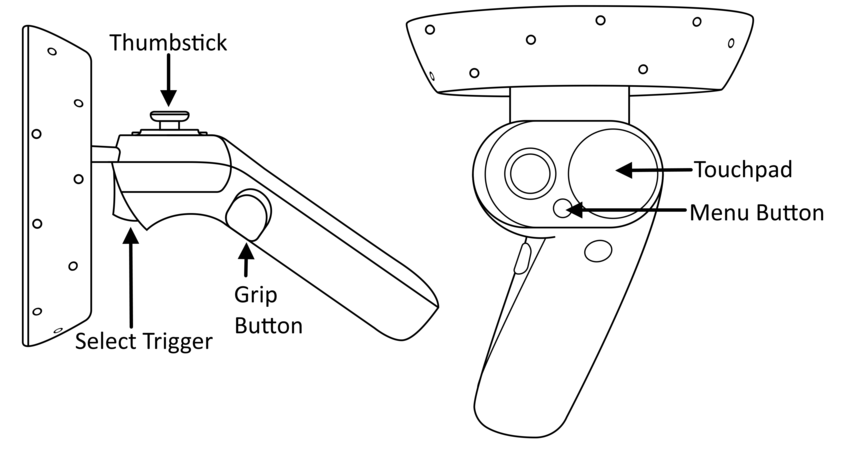
\includegraphics[scale=.35]{hpController.png}
\end{center}

The HP Microsoft Mixed Reality Controllers are wireless controllers that support inside-out tracking, and thus require less initial set up than the other outside-in tracking systems. A lack of required setup time is good, but there are downsides; slightly more latency and the fact that the controllers will not be tracked if the user is not looking at them and they are not in the headset mounted camera view. The controllers are in between the Vive controllers and Oculus Touch in terms of weight and size, and have a slightly lower build quality. They have a trackpad, analogue stick, triggers, grip buttons, and a menu button.

\subsubsection{Vive Controller}
\begin{center}
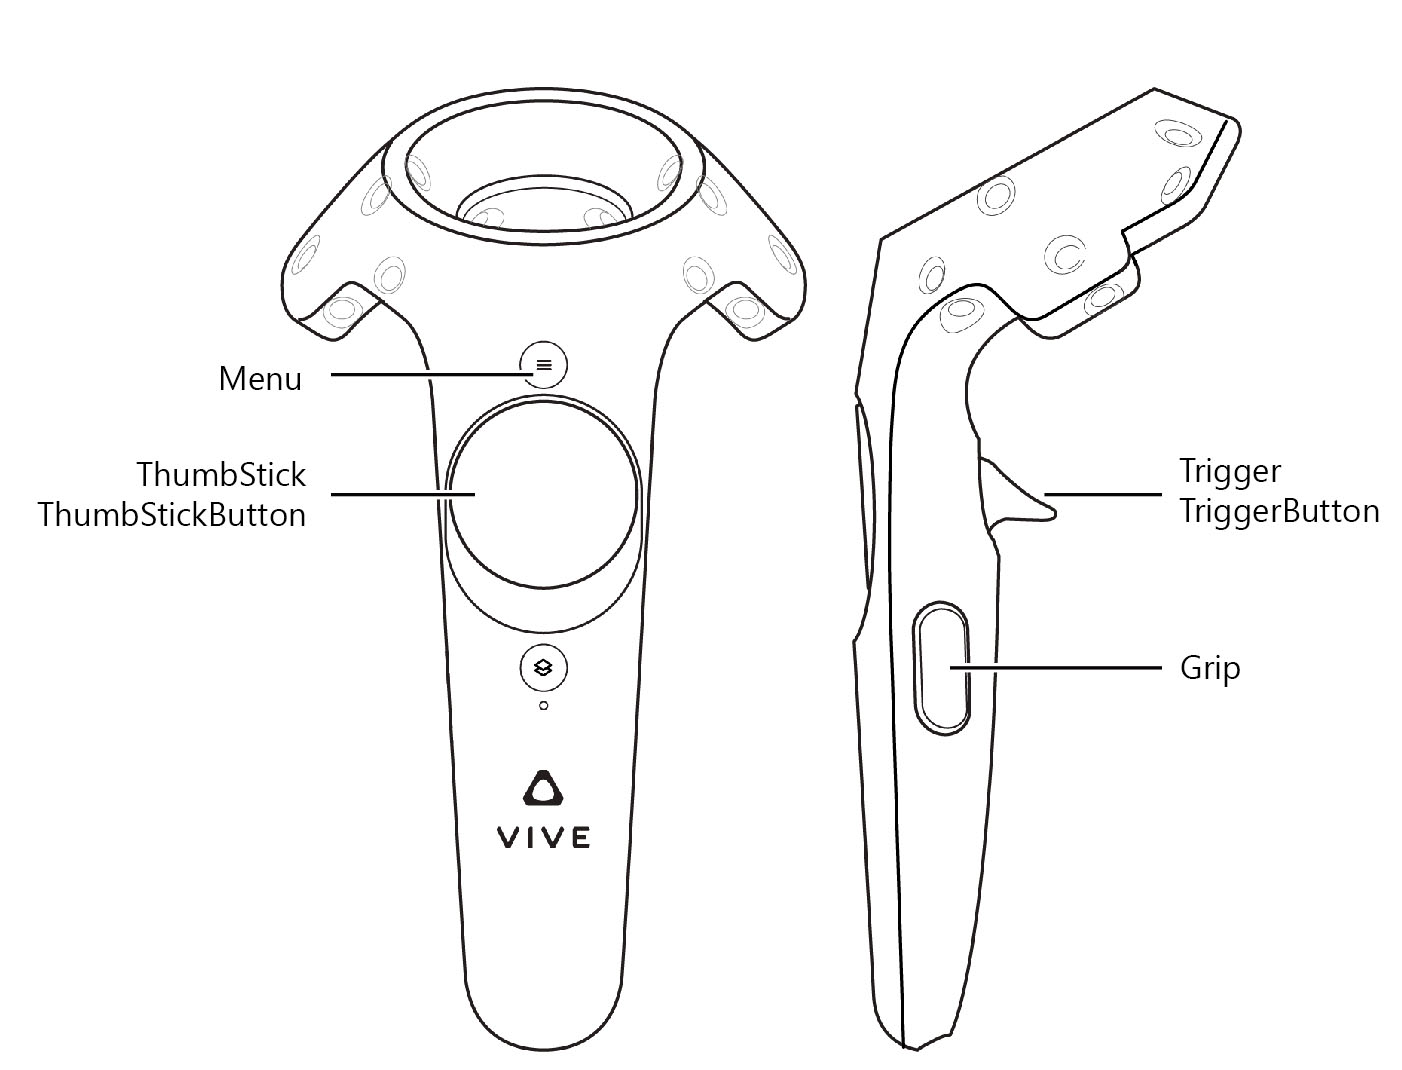
\includegraphics[scale=.20]{viveController.jpg}
\end{center}

The Vive controllers sport wireless controllers that contain rechargeable lithium ion batteries. These controllers have circular touchpad buttons for thumbs, a side mounted grip button, a menu button, a system button, and a trigger on the underside of the controller. Vive controllers are the heaviest and potentially the most unwieldy, due to their overall large size. The controllers also support room scale VR, meaning that the player can actually walk around the room and the camera system will track their position, moving them in the virtual world. 

\subsubsection{Oculus Touch}
\begin{center}
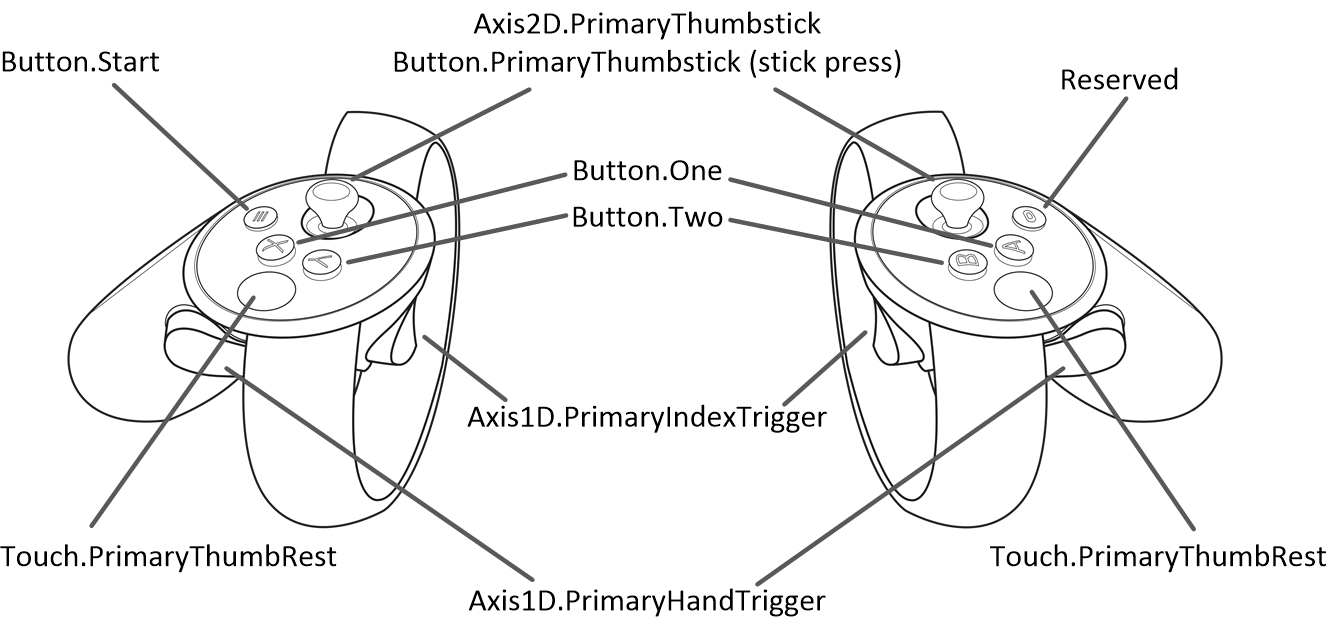
\includegraphics[scale=.30]{oculusController.png}
\end{center}

The Oculus Touch controllers are generally regarded as the best virtual reality controllers currently on the market. They are lightweight and natural feeling, have the best finger tracking around, and have a sleek appearance. One controller is about half the size of a modern gamepad, has two letter buttons, an analogue stick, two triggers, menu and start buttons, a set of buttons on the grip, and a touch sensor for the thumb next to the joystick \cite{controllerCompare}. Having more inputs than any other controller allows the Oculus touch to allow users to have more complex interactions with virtual environments. These controllers are also wireless and require AA batteries. The controllers require the use of a camera sensor and thus an additional USB 3.0 port. During initial setup the user is required to use their motion controllers and the sensors to map the play space, the area that the virtual reality system will allow to player to act in. 

% VRUIs (Virtual Reality User Interfaces)
% VRGUIs (Virtual Reality Graphical User Interfaces)
\section{User Interface (UI)}
User interface is a broad topic and can be applied to many fields, but here we will be talking about UI as it is used in video games and other virtual reality applications. 

% What they are and how they relate to VR
\subsection{Types of user interfaces}

\subsubsection{Non-diegetic}
The term non-diegetic is generally used in terms of sounds in film, where a non-diegetic sound is a sound whose source is not visible on screen or has not been implied to be present in the action. Non-diegetic UI is generally a UI element or elements that are overlaid on top of the screen to show things like menus, health bars, or other elements that must be view-able and/or intractable by the user. This type of UI is often referred to as Heads Up Display (HUD) in games. Non-diegetic UI does not particularly work in virtual reality, because overlaying something in front of the screen display forces UI elements too close to the eye to be able to focused on.    

\subsubsection{Spatial UI}
Spatial UI refers to placing UI "in the world", allowing our eyes to focus on the UI element \cite{unity}. In virtual reality this means that UI lives in the same space as any other objects in the VR scene. This type of UI may need to be scaled according to user position, and may be scaled dynamically. A best practice is to position UI elements at a distance that is comfortable for reading, and scaling the elements based on how far away the user is at any given time. Spatial UI elements are often attached to the camera, so the element will stay fixed in the player view.

\subsubsection{Diegetic UI}
Diegetic UI is having elements in the world environment display information to the user. This could refer to things such as in world screens and holographic displays attached to objects. The main difference between spatial UI and diegetic UI is that spatial UI is based on where the user is looking, and diegetic UI is often attached to a non-player object and is independent of player view.  

\section{Conclusion}
After researching virtual reality headsets, motion controllers, and user interface schemes, I believe that our project would be best served by using the Oculus Rift, the Oculus Touch controllers, and mostly diegetic UI with some spatial UI elements. As of this writing Oculus virtual reality products represent the cutting edge consumer hardware in the field and we would be best served by developing on this hardware. That being said, our client works with HP and the end product will most likely be used with the HP Microsoft Mixed Reality headset and controllers. This means that while we may do most development with Oculus hardware, we must also consider the fact that the end product must also run on the HP headset. At this point I do not believe that this will be a problem, as most VR applications written with commercial game engines, such as Unreal, are headset agnostic. We must be aware of hardware specific features though, and make sure nothing we implement requires a feature of a headset and controller combination that another may not support. 

\bigskip
\begin{thebibliography}{999}

\bibitem{headsetCompare}
  J. Newman and B. Cross,
  'HTC Vive vs. Oculus Rift vs. Windows Mixed Reality: What's the difference?',
  2018.
  [Online].
  Available: https://www.pcworld.com/article/3223202/virtual-reality/htc-vive-vs-oculus-rift-vs-windows-mixed-reality.html
  [Accessed: 10-31-2018]

\bibitem{controllerCompare}
  N. Pino,
  'Oculus Touch',
  2017.
  [Online].
  Available: https://www.techradar.com/reviews/oculus-touch-controller
  [Accessed: 11-2-2018]

\bibitem{unity}
  Unity,
  'User Interfaces for VR'.
  [Online].
  Available: https://unity3d.com/learn/tutorials/topics/virtual-reality/user-interfaces-vr
  [Accessed: 10-31-2018]
 
\end{thebibliography}

\end{document}